\documentclass{standalone}
\usepackage{tikz}
\usetikzlibrary{matrix,decorations.pathreplacing,arrows}

\begin{document}
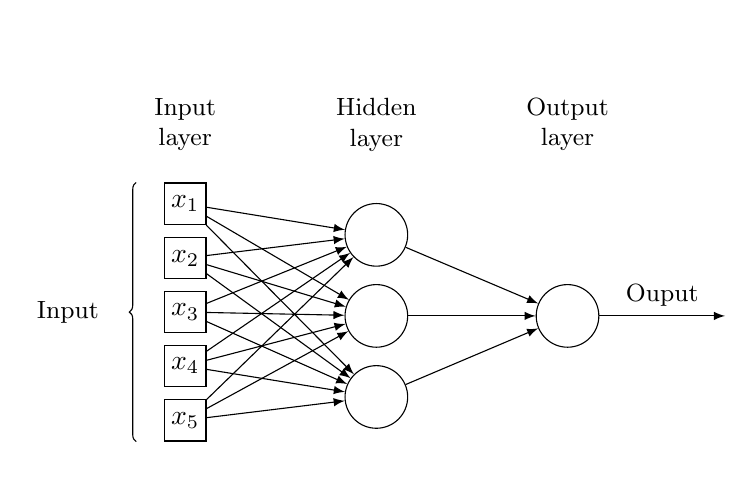
\begin{tikzpicture}[
  plain/.style={
    draw=none,
    fill=none,
    font=\small
  },
  input/.style={
    draw,
    rectangle,
    fill=none,
    minimum width=1.5em,
    minimum height=1.5em,
    inner sep=0pt
  },
  net/.style={
    matrix of nodes,
    nodes={
      draw,
      circle,
      inner sep=8pt
    },
    nodes in empty cells,
    column sep=0.2cm,
    row sep=-13pt
  },
  >=latex
]

\matrix[net] (mat) {
  % Text row
  |[plain]| \parbox{1.3cm}{\centering Input\\layer} &
  |[plain]| \parbox{1.3cm}{\centering Hidden\\layer} &
  |[plain]| \parbox{1.3cm}{\centering Output\\layer} \\
  % Nodes
  |[input]| $x_1$ & |[plain]| & |[plain]| \\
  |[plain]|       &           & |[plain]| \\
  |[input]| $x_2$ & |[plain]| & |[plain]| \\
  |[plain]|       & |[plain]| & |[plain]| \\
  |[input]| $x_3$ &           & \\
  |[plain]|       & |[plain]| & |[plain]| \\
  |[input]| $x_4$ & |[plain]| & |[plain]| \\
  |[plain]|       &           & |[plain]| \\
  |[input]| $x_5$ & |[plain]| & |[plain]| \\
};

% Arrows 1
\foreach \ai in {2,4,...,10} {
  \foreach \aii in {3,6,9} {
    \draw[->] (mat-\ai-1) -- (mat-\aii-2);
  }
}

% Arrows 2
\foreach \ai in {3,6,9} {
  \draw[->] (mat-\ai-2) -- (mat-6-3);
}

% Arrow 3
\draw[->] (mat-6-3) -- node[above] {\small Ouput} +(2cm,0);

% Brace
\draw[decorate,decoration={brace,mirror,raise=10pt}]
  (mat-2-1.north west) -- node[left=20pt] {\small Input} (mat-10-1.south west);

\end{tikzpicture}
\end{document}
